\documentclass[a4paper,oneside]{book} 
% the 'oneside' option makes viewing on a computer easier, as both inner and outer margins are equal. Change this while printing.

\usepackage{amsmath,amssymb}
\usepackage[linkbordercolor={0.9 0.9 1}]{hyperref}
\usepackage{amscd}
\usepackage{amsthm}
\usepackage{color}

\usepackage[T1]{fontenc}

\usepackage{enumerate} % Customize the enumerate environment
\usepackage{mathtools} % for \prescript

%\usepackage{cite}
\usepackage{bm} 

\usepackage[vcentermath]{youngtab} % Excellent package for young diagrams

% For compact lists. Provides the environments 
%   itemize*, enumerate*, description*
% with lesser spacing between items.
\usepackage{mdwlist} 
\usepackage{enumerate} 

\usepackage{mathtools} % For 'Aboxed' command

% Theorem-like environments
\usepackage{amsthm}
\theoremstyle{definition}
\newtheorem{definition}{Definition}

\theoremstyle{plain}
\newtheorem{theorem}{Theorem}
\newtheorem{corollary}{Corollary}
\newtheorem{conjecture}{Conjecture}
\newtheorem{lemma}{Lemma}
\newtheorem{proposition}{Proposition}

% TikZ
\usepackage{tikz}
\usepackage{tikz-cd} % Commutative Diagrams in TikZ
\usetikzlibrary{positioning}
\usetikzlibrary{decorations.pathreplacing} % for curly braces
\usetikzlibrary{decorations.pathmorphing} % for squiggly arrows
\usetikzlibrary{calc} % for coordinate calculation
% Tikz Style for Commutative Diagrams
\tikzset{
    commutative diagram/.style={
            node distance=2cm,auto,
            arrow/.style={-stealth},
            exists/.style={-stealth,densely dotted}
        }
    }

% This compactifies a list by removing unnecessary whitespace
\newcommand\makethislistcompact{
        \setlength{\itemsep}{0pt}%
        \setlength{\parskip}{0pt}%
        %\setlength{\topsep}{50pt} 
        %\setlength{\partopsep}{10pt}
        %\setlength{\parsep}{50pt}
}
% Framed environments
\usepackage[framemethod=tikz]{mdframed}

% Common operators
\DeclareMathOperator\GL{GL}  % General Linear Group
\DeclareMathOperator{\Image}{Im} % Image
\DeclareMathOperator{\Coker}{Coker} % Cokernel 
\DeclareMathOperator{\Ker}{Ker} % Kernel
\DeclareMathOperator{\Tr}{Tr} % Trace
\DeclareMathOperator{\Hom}{Hom} % Homomorphisms
\DeclareMathOperator{\End}{End} % Endomorphisms
\DeclareMathOperator{\Aut}{Aut} % Automorphisms
% Commonly used sets
\newcommand{\CC}{\mathbb{C}}
\newcommand{\RR}{\mathbb{R}}
\newcommand{\ZZ}{\mathbb{Z}}
\newcommand{\HH}{\mathbb{H}}
\newcommand{\FF}{\mathbb{F}}
\newcommand{\uhp}{\mathcal{H}}
\newcommand{\SL}{\text{SL}}

\renewcommand{\>}{\rangle}
\newcommand{\<}{\langle}

% Some semantically named symbols
\newcommand\isomorphic\cong

% Meta-notes
\newcommand\Solution[2]{\emph{[Solution to Exercise #1 in #2]}}
\newcommand\Todo[1]{\begin{color}{red}{#1}\end{color}}
\newcommand{\tocheck}[1]{{\color{red} #1}}
\newcommand{\comment}[1]{{\color{cyan} #1}}

% Environment for "physical insights"
\newenvironment{insight}
  {\begin{mdframed}[%style=2,%
      leftline=true,
      rightline=true,
      topline=false,
      bottomline=false,
      leftmargin=2em,
      rightmargin=2em,%
      innerleftmargin=1em,
      innerrightmargin=1em,
      linewidth=2pt,%
      linecolor=white!70!black,%
      %backgroundcolor=white!99!black, %
      skipabove=7pt,skipbelow=7pt]\small}
  {\end{mdframed}}

%%%%%%%%%%%%%%%%%%%%%%%%%%%%%%%%



% Bibliography using BibLaTeX/Biber
\usepackage[
    backend=biber,
    style=alphabetic,
    sortlocale=en_US,
    hyperref=true,
    url=true, 
    doi=true,
    eprint=false
]{biblatex}
\addbibresource{repth.bib}

\usepackage[vcentermath]{youngtab} % Excellent package for young diagrams
\setcounter{secnumdepth}{1}

% Some common representations
\DeclareMathOperator{\Sym}{Sym} % Symmetric product
\DeclareMathOperator{\Alt}{\Lambda} % Exterior product
\DeclareMathOperator{\sgn}{sgn} % Alternating representation
\DeclareMathOperator{\triv}{triv} % Trivial representation
\DeclareMathOperator{\std}{std} % Standard representation
\DeclareMathOperator{\Ind}{Ind} % Induced representation 

% Some common maps
\DeclareMathOperator{\id}{id}

\DeclareMathOperator{\gr}{gr}

\DeclareMathOperator{\ad}{ad}

% Semantic stuff
\newcommand{\injects}{\hookrightarrow}
\newcommand{\onto}{\twoheadrightarrow}
\newcommand{\germs}{\mathcal E}
\newcommand{\defn}[1]{\textbf{#1}}
\newcommand\Weyl{\mathcal{W}}

% Some common lie algebras
\newcommand{\Lie}[1]{\mathfrak{\lowercase{#1}}}
\newcommand{\LieGL}{\mathfrak{gl}}
\newcommand{\LieA}{\mathfrak{a}}
\newcommand{\LieB}{\mathfrak{b}}
\newcommand{\LieG}{\mathfrak{g}}
\newcommand{\LieH}{\mathfrak{h}}
\newcommand{\LieSL}{\mathfrak{sl}}

% Some common lie algebra ideals
\DeclareMathOperator\Rad{Rad}


\DeclareMathOperator\height{ht}

%%%%%%%%%%%%%%%%%%%%%%%%%%%%%%%%

% Title
\title{Representation Theory}
\author{Hersh Singh}
\begin{document}
\maketitle

\tableofcontents

\chapter{Representations of Finite Groups}
\section{Definitions}
\label{sec:definitions}

Let $G$ be a finite group, $V$ be a finite dimensional complex vector space.

A \emph{representation} of $G$ on $V$ is a group homomorphism 
\begin{align}
    \rho:  G\to \GL(V), 
\end{align}
where $\GL(V)$ is the group of automorphisms of $V$. Even though the ``representation" is really the vector space $V$ \emph{and} the homomorphism $\rho$, but it is common (especially by physicists) to refer to $V$ itself as the representation. 

\begin{insight}
We say that this map gives $V$ the structure of a G-module. This agrees with the  definition of a R-module (R is a ring) that I have studied earlier. An R-module is simply a vector space defined over a ring, instead of a field. So the ring elements act as the \emph{scalars}. Of course, the description must include a rule for the `interaction' of the scalars with the vectors. To be a module, the interaction must be \emph{linear}.  
In this case, the group homomorphism $\rho$ gives us that rule of interaction between the vectors (elements of $V$) and the scalars (elements of $G$). For $g\in G, v \in V$, $$gv\equiv\rho(g)v \in V$$
\end{insight}


A vector space homomorphism $\phi: V\to W$ is a morphism between the two representations $V$ and $W$ if the following diagram commutes:
\begin{equation} \begin{CD}
  V @>\phi>> W\\
  @VgVV @VVgV\\
  V @>\phi>> W\\
\end{CD} \end{equation}

That is, $\phi g=g\phi$ for all $g\in G$. This makes the group elements \emph{behave like scalars under module homomorphisms}. Such morphisms of representations are also called $G$-\emph{linear map} or a \emph{$G$ intertwiner}.

\begin{insight}
   Why is this is a good definition? Seems to be inspired from module homomorphisms. This is natural in some sense - Figure that out.
\end{insight}

$\Ker \phi,\ \Image \phi,\ \Coker \phi = V/\Image\phi$ are also $G$-modules. This is solely because of the commutativity of the above diagram.
\begin{itemize}
    \item If $v\in \Ker \phi$, then $\phi(gv) = g\phi(v) = 0$. So $gv$ also $\in \Ker \phi$. $\blacksquare$.
    \item If $v\in \Image \phi$, then let $\phi(v) = w$. So $\phi(gv)=g\phi(v)=gw \in W$. So $gv$ also $\in \Image \phi$. $\blacksquare$.
\end{itemize}

One of the goals of our study is, given a representation, to develop tools for constructing other, preferably all, representations of the group. 
Some examples of representations that can be constructed from $V$ and $W$

\begin{enumerate}[(a)]
    \item Tensor product $V\otimes W$ via
        \begin{align}
            g(v\otimes w) = g(v) \otimes g(w)
        \end{align}
    \item Tensor power $V^{\otimes n}$ and the \emph{exterior power}  $\Lambda^n(V)$ and the \emph{symmetric power} $\Sym^n(V)$ are its subrepresentations.
    \item the dual $V^* = \Hom(V,\CC)$. This is a little tricky though. The action of $G$ on $V^*$ must be such that it preserves the natural inner product, denoted by $\<\ ,\ \>$, between them. So, if we have a representation $(V^*,\rho^*)$ and $(V,\rho)$, then we should have
        \begin{align}
            \rho^*_g(u^*)(\rho_g v) = u^*(v)
        \end{align}
        where I have written $\rho_g=\rho(g)$ for a cleaner notation, and $u^*\in V^*,\ v\in V$. 
        \begin{insight}
            Remember the definition of the transpose map. If we have a map $f: V\to W$, then the transpose of $\rho$ is a map $^t\rho: W^*\to V^*$ such that
            \begin{align}
                ^tf(\phi) = f\cdot \phi \quad\quad\forall \phi\in W^*.
            \end{align}
            It's a good idea to make commutative diagrams out of statements like the above:
            \begin{center}
            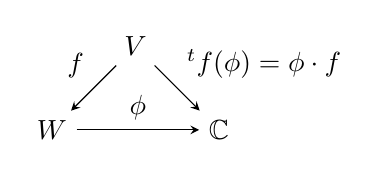
\begin{tikzpicture}[commutative diagram, node distance=1.5cm]
                \node (V) {$V$};
                \node (CC) [below right of=V] {$\CC$};
                \node (W) [below left of=V] {$W$};
                \draw [arrow] (V) -- (CC) node [midway] {$^tf(\phi)=\phi\cdot f$};
                \draw [arrow] (V) -- (W) node [midway,auto=right] {$f$};
                \draw [arrow] (W) -- (CC) node [midway] {$\phi$};
            \end{tikzpicture}
            \end{center}
        \end{insight}
        If we now define
        \begin{align}
            \rho^*(g) &= \prescript{t}{}\rho(g^{-1})
            \label{eqn:defn_dualrep}
        \end{align}
        we get
        \begin{align*}
            \rho_g^*(u*)(\rho_g v) &= \prescript{t}{}\rho_{g^{-1}}(u^*)(\rho_g v)\\
                &= u^*\cdot\rho_{g^{-1}} (\rho_g v) \\
                &= u^* (\rho_{g^{-1}g} v) \\
                &= u^*(v).
        \end{align*}
        The definition \eqref{eqn:defn_dualrep} preserves the inner product, and is a thus a sane definition.
    \item $\Hom(V,W)$ by the identification, $\Hom(V,W)=V^*\otimes W$ (see appendix \ref{cha:tensor_product}). If $(\phi: V\to W)\in \Hom(V,W)$ then let $\sum_i \phi_{ij} v_i^*\otimes w_j$. Writing out the action of this on $u\in V$,
        \begin{align*}
            (g\phi)(gu) &= \left[ g \sum\phi_{ij} v^*_i \otimes w_j \right] (gu) \\
                &= \Big[ \sum_{ij}\phi_{ij} gv^*_i \otimes gw_j \Big] (gu) \\
                &= \sum \phi_{ij} \<gv_i^*, gu\> g w_j\\
                &= \sum \phi_{ij} \<v_i^*, u\> g w_j\\
        \end{align*}
        This gives us
        \begin{align}
            (g\phi)(gu) &= g\cdot\phi(u)\quad \forall u\in  V.
            \label{eqn:linearmap_groupaction}
        \end{align}
        \begin{insight}
            Note that you cannot multiply both sides by $g^{-1}$ to imply that $\phi(gu)=\phi(u)$. This can't be done since the action of $G$ on $V^*$ is \emph{not associative}. That means,
            \begin{align*}
                (g\phi)(u) \neq g\cdot \phi(u),
            \end{align*}
            as can be seen by simply taking, say, $\phi=v^*\otimes w$. LHS becomes $\< gv^*, u \>gw$ while RHS becomes $\<v^*,w\>gw$.
        \end{insight}
        \begin{center}
            \begin{tikzpicture}[commutative diagram]
                \node (V1) {$V$};
                \node (W1) [right of=V] {$W$};
                \node (V2) [below of=V1] {$V$};
                \node (W2) [below of=W1] {$W$};
                \draw [arrow] (V1) -- (W1) node [midway, auto=right] {$\phi$};
                \draw [arrow] (V2) -- (W2) node [midway, auto=right] {$g\phi$};
                \draw [arrow] (V1) -- (V2) node [midway, left] {$g$};
                \draw [arrow] (W1) -- (W2) node [midway] {$g$};
            \end{tikzpicture}
        \end{center}
        Of course, if $\phi$ is a $G$-linear map (a map between representations $V$ and $W$), then we also have $g\cdot\phi = \phi\cdot g$ for all $g\in G$. Consider the space $\Hom_G(V,W) \subset \Hom(V,W)$, which consists of maps from $V$ to $W$ invariant under the action $G$. If $\phi\in \Hom_G(V,W)$, then we have $(g\phi)(gu)=g\phi(u)$ and $(g\phi)(u)=\phi(u)$ (by invariance of the map under $G$). Thus we have $g\phi(u)=\phi(gu)$. The converse is also easily seen to be true.Therefore, $\Hom(V,W)$ is space of all $G$-linear maps $V\to W$.  \Solution{1.2}{FH} 

        
\end{enumerate}



\begin{itemize}
    \item \Todo{Todo: Regular Representation}
    \item \Todo{Exercise 1.3,1.4}
\end{itemize}

\section{Schur's Lemma}
\label{sec:schur_s_lemma}

\begin{lemma}[Schur's Lemma]
    Let $V,\ W$ be irreps of a group $G$ and $\phi: V\to W$ a $G$-linear map. Then,
    \begin{enumerate}[(i)]
        \item either $\phi$ is 0 or an isomorphism;
        \item if $V=W$, then $\phi=\lambda I$.
    \end{enumerate}
\end{lemma}

\section{Examples}
\label{sec:examples}

We observe that any $g\in G$ gives a map $\rho(g): V\to V$. In general, this is not a $G$-linear map however. For $\rho(g)$ to be a $G$ linear map, ...
%\begin{align}
    %g(h(v)) &= h(g(v))\quad\quad \forall h\in G
%\end{align}
%which just says that the set of all $G$-linear maps in $\rho(G)$ is precisely the center of $G$, given by $Z(G)$.

\subsection{Abelian Groups}
\label{sub:abelian_groups}

If $G$ is an abelian group, and $V$ is an irrep, then $\rho(g)$ is a $G$-linear map.By Schur's Lemma, $\rho(g)=\lambda I$. That means that any proper subspace of $V$ is actually invariant under the action of $G$, and is a thus a subrepresentation. But since $V$ is irreducible, this can only mean that $V$ has no non-trivial proper subspace, which implies that $V$ is one-dimensional. Therefore, any representation of an abelian group is just an element of the \emph{dual group}
\begin{align}
    \rho: G \to \CC^*.
\end{align}

%Incidentally, this is also the definition of the \emph{dual group}.

\subsection{\texorpdfstring{$S_3$}{S3}}
%\label{sub:_s_3_}

\begin{insight}
    Remember that $S_3$ is the group of permutations of three objects. Algebraically, it can be thought to be generated by the elements
    \begin{align}
        \{1,\ \tau,\ \tau^2, \sigma,\ \sigma\tau,\ \sigma\tau^2\}
    \end{align}
    subject to the conditions
    \begin{align}
        \tau^3=1,\quad \sigma^2=1,\quad (\sigma\tau)^2=1.
    \end{align}
    You can tell that $\sigma$ is a 2-cycle and $\tau$ is a 3-cycle.
    
\end{insight}

Lets now discuss the case of the \emph{simplest non-abelian group}, $S_3$. We already know three representations to begin with:
\begin{enumerate}[(i)] 
    \makethislistcompact
    \item the trivial representation,
        \begin{align}
            \rho(g) &= I
        \end{align}
    \item the alternating representation
        \begin{align}
            \rho(g) &= \sgn(g),
        \end{align}
    \item the natural permutation representation.\\
        But this is not irreducible. It can be easily seen that the subspace spanned by the vector $(1,1,1)$ is invariant under $G$. So, the space $V$ complimentary to it is another (hopefully irreducible!) representation. If $v=(z_1,z_2,z_3) \in V$, then 
        \begin{align}
            (z_1,z_2,z_2)\cdot(1,1,1) &= 0\\
            \implies z_1 + z_2 + z_3 &= 0.
        \end{align}
        We thus have
        \begin{align}
            V &= \{(z_1,z_2,z_3) \in \CC^3: z_1 + z_2 + z_3 =0\}.
        \end{align}
        Now if this further has an invariant subspace, it must be spanned by an element of the form $(z_1,z_2,-z_1-z_2)$. Applying a few permutations will convince you immediately that this is not an invariant subspace. Therefore, the representation we have is irreducible, called the \emph{standard representation} of $S_3$.
\end{enumerate}
We now want to characterize any arbitrary representation $W$ of $S_3$. To do so, we first look at the action of the abelian subgroup $ U_3 = \ZZ/3 \in G$ (generated by $x$) on $W$. If $v\in W$ is an eigenvector of $\rho(x)$, then 
\begin{align}
    \tau \sigma (v) &= \sigma\tau^2 (v)\\
        &= \omega^2 (\sigma v)
\end{align}
This means that if $v$ is eigenvector of $\tau$ with the eigenvalue $\omega$, then $\sigma v$ is also an eigenvector with the eigenvalue $\omega^2$.
To find the decomposition of the $W$, we go through the following steps:
\begin{enumerate}[(i)]
    \item Start with an eigenvector $v$ of $\tau$, which has the eigenvalue $w^i$.
    \item If $w^i\neq 1$, then $\sigma v$ is an eigenvector independent of $\tau$ with the eigenvalue $w^{2i}$. In this case, $\{v,\sigma v\}$ form a two dimensional subspace of $W$ invariant under $S_3$ (as $\sigma$ just exchanges $v$ and $\sigma v$). In fact, this subrepresentation is isomorphic to the standard representation and is thus irreducible.
    \item If $w^i = 1$, then $\sigma v$ may or may not be independent of $v$.
        \begin{enumerate}
            \item If $\sigma v$ is independent of $v$, then $v + \sigma v$ spans a subspace isomorphic to the trivial representation and $v - \sigma v$ spans a subspace isomorphic to the alternating representation. 
            \item If $\sigma v$ and $v$ are not linearly independent, then 
                $\sigma v= \lambda v$ for some $\lambda\in \{1,-1\}$ (since $\sigma^2=I$). If $\lambda=1$, then $\CC v$ is isomorphic to the trivial representation and if $\lambda=-1$, then $\CC v$ is isomorphic to the alternating representation.
        \end{enumerate}
\end{enumerate}

Note that this allows to find all irreps of a given representation $W$!

\Solution{1.12(a)}{FH} Lets use this approach to find out the irreps of th regular representation $R$ of $S_3$. A general vector in the space looks like this
\begin{align}
    v &= a_1 + a_2 \tau + a_3 \tau^2 + b_1\sigma + b_2 \sigma\tau + b_3\sigma \tau^2 
\end{align}

The eigenvalues of $\tau$ are $\{1,\omega,\omega^2\}$. 
\begin{enumerate}
    \makethislistcompact
    \item For eigenvalue $=1$, we have $v=1 + \tau + \tau^2$ and $\sigma v = \sigma + \sigma\tau + \sigma\tau^2$. Thus $\CC (v+\sigma v)\isomorphic \triv$ and $\CC (v-\sigma v) \isomorphic \sgn$ are two irreps.
    \item For eigenvalue $=\omega$, we get on solving $\tau \alpha = \omega \alpha$
        \begin{align}
            \alpha &= \omega^2\tau + \omega\tau + \tau^2
        \end{align}
        With $\beta = \sigma \alpha$, we get the subspace spanned by $\{\alpha,\beta\}$ to be isomorphic to the standard representation.
    \item For eigenvalue $=\omega^2$, we get 
        \begin{align}
            \alpha' &= \omega^2 + \omega\tau + \tau^2\\
            \beta' = \sigma\alpha &= \omega^2\sigma + \omega\sigma\tau + \sigma\tau^2
        \end{align}
        The subspace spanned by $\{\alpha',\beta'\}$ is again isomorphic to the standard representation.
\end{enumerate}
We have enumerated six linearly independent eigenvectors and therefore exhausted all of them. We thus get
\begin{align}
   R &\isomorphic \triv \oplus \sgn \oplus (\std)^2 \quad\quad\square    
\end{align}
\Solution{1.14}{FH} For an irrep $V$ of a finite group $G$, there is a unique Hermitian inner product preserved by $G$. Say there are two Hermitian products, $H$ and $H'$, preserved by $G$. Any Hermitian inner product sets up an isomorphism between $V$ and $V^*$. Let that map be given by
\begin{align}
    \phi_1(v) &= H_1(v,\cdot) \in V^*\\
    \phi_2(v) &= H_2(v,\cdot) \in V^*
\end{align}
\begin{insight}
    Write details about the isomorphism between $V$ and $V^*$. Crucial is the positive-definiteness of the inner product. Not sure where the Hermiticity of the inner product is important.
\end{insight}
\begin{align}
    V^* \xleftarrow{\phi_1} V \xrightarrow{\phi_2} V^*
\end{align}
Now, the map $\phi = \phi_2\cdot\phi_1^{-1}$ is an isomorphism of vector spaces. It is also a $G$-linear map since its the composition of $G$-linear maps. Therefore, $\phi$ is an isomorphism between two irreps. By Schur's lemma, $\phi=\lambda\cdot I$, where $\lambda$ is any scalar. This gives us
\begin{align}
    H_2(v,\cdot) &= \phi(H_1(v,\cdot)) \\
        &= \lambda H_1(v,\cdot)\quad\quad\qed
\end{align}

\noindent\Todo{\Solution{1.13(a)}{FH}}\\
\Solution{1.13(b)}{FH} Is $\Sym^n(\Sym^mV)\isomorphic \Sym^m(\Sym^n V)$? No, since the dimensions don't match on both sides.
\begin{align}
    \dim \Sym^n(\Sym^mV) &= ^{{}^{\dim V - 1 + m}C_{m} -1 +n}C_{n}
\end{align}
The above equation is clearly not symmetric in $m$ and $n$. So the isomorphism can not hold in general.


\chapter{Character Theory}
\label{cha:character_theory}
\begin{definition}
    If $V$ is a representation of $G$, its \emph{character} $\chi_V$ is the complex-valued function on the group defined by
    \begin{align}
        \chi_V(g) &= \Tr(g|_V),
    \end{align}
    the trace of $g$ on $V$.
\end{definition}

We shall drop the subscript $V$ when it's obvious.

Some properties
\begin{enumerate}
    \item $\chi_V$ is a class function, which means that it is constant on conjugacy classes  of $G$.
        \begin{align}
            \chi(hgh^{-1}) &= \chi(g)
        \end{align}
    \item 
\end{enumerate}

\section{First Projection Formula}
\label{sec:first_projection_formula}
Let us define $V^G$ as the elements of $V$ fixed under the action of $G$.
\begin{align}
    V^G=\{v\in V: gv=v\ \forall g\in G \}
\end{align}
The sub space $V^G$ is actually the direct sum of the trivial subrepresentations.

Now, the endomorphism $\varphi \in \End(V)$, 
\begin{align}
    \varphi &= \frac{1}{|G|} \sum_{g\in G} g
\end{align}
is $G$ linear, since $h\varphi h^{-1} = \frac{1}{|G|}\sum_{g\in G} hgh^{-1} = \varphi$.  Infact, $\varphi$ is projection of $V$ to $V^G$.

So, now we have a way of finding the direct sum of the trivial subrepresentations of $V$. The trace of this map is would be the dimension of $V_G$ [\Todo {Why?}], which is the number of copies of trivial representations in $V^G$.

\begin{insight}
    \Todo{ For an arbitrary linear map (projection?) $T: V\to W$, do we have $\Tr T =\dim W$ ?  }
\end{insight}

\begin{align}
    \dim V^G &= \Tr (\varphi)\\
        &= \frac{1}{|G|}\sum_{g\in G} \Tr(g)\\
        &= \frac{1}{|G|}\sum_{g\in G}\chi_V(g)
        \label{eqn:dimV_G}
\end{align}
In particular, if $V$ is irreducible, then it has no trivial subrepresentations and thus
\begin{align}
    \sum_{g\in G} \chi_V(g) &= 0\quad\quad\text{if $V$ is an nontrivial irrep}.
\end{align}

We know that $\Hom(V,W)^G$, the set of all homomorphisms $V\to W$ fixed under $G$, is just the space of all $G$-linear maps $V\to W$. [\Todo{reference here.}]
\begin{insight}
    Given a $G$-linear map $\phi: V\to W$, where $V$ is an irrep, $\phi$ defines an isomorphism between $V$ and $\Image(\phi)$ (since $\ker \phi$ is a subrepresentation of $V$, and so must be $\{0\}$) Now, other such $\phi$ would give us copies of $V$ in $W$. \Todo{The dimensionality of the space $\Hom_G(V,W)$ thus tells us the multiplicity of $V$ in $W$.}
\end{insight}

By Schur's lemma, if $V$ and $W$ are both irreducible then
\begin{equation}
    \dim \Hom_G(V,W) = 
        \begin{cases}    
            1   &\text{if } V\isomorphic W \\
            0   &\text{if } V\ncong  W
        \end{cases}
\end{equation}
Since we have $\Hom_G(V,W)\isomorphic V^*\otimes W$,
\begin{align}
    \chi_{\Hom_G(V,W)}(g) &= \overline{\chi_V(g)}\cdot\chi_W(g)
\end{align}
Using \eqref{eqn:dimV_G} here, we get the nice result
\begin{align}
        %\frac{1}{|G|}\sum_{g\in G}\chi_V(g) &= 
        \frac{1}{|G|}\sum_{g\in G} \overline{\chi_V(g)}\cdot\chi_W(g) 
        &= \begin{cases}    
            1   &\text{if } V\isomorphic W \\
            0   &\text{if } V\ncong  W
        \end{cases}
\end{align}
This inspires us to define a dot product on the space of all class functions (functions that are defined on the conjugacy classes of a group) of $G$,
\begin{align}
    \CC_{\text{class}}(G) &= \{\text{class functions on $G$}\},
\end{align}
as
\begin{align}
    (\alpha,\beta) &= \frac{1}{|G|} \sum_{g\in G} \overline{\alpha(g)} \beta(g).
    \label{eqn:dotproduct_classfunctions}
\end{align}
In respect this dot product, the characters of irreps are orthonormal.

\chapter{Induced Representations}
\label{cha:induced_reprentations}

This chapter is based heavily on \cite{etingof_introduction_2009}.
\section{Overview}
\begin{enumerate}
    \makethislistcompact
    \item Define induced representations
    \item Mackay formula for the character of an induced representation.
    \item Frobenius Reciprocity
\end{enumerate}

\section{Definitions}

\Todo{Don't really understand the motivation for this section.}

Given a subgroup $H\subset G$, and $(\rho_V, V)$, a representation of $G$, we can easily construct a representation for $H$ by simply restricting $\rho_V$ to $H$, which we denote by $\rho_V|_H$.

However, if want to construct a representation of $G$ from a representation of $H$, then we need to think a little more about it. 

Think of the elements of $V$ as functions of $G$, that is, every element $v\in V$ defines a map $v: G\to V$ given by
\begin{align}
    v(g) &= \rho(g) v.
\end{align}
Now, we already know how $v(\cdot)$ acts on $H$. We want to extend that action to $G$. The least we could do is to ensure that the action on $G$ is consistent with the known action on $H$. So, we enforce that
\begin{align}
    v(hg) = h\cdot v(g) &= \rho_V(h) v(g)\quad \forall h\in H,\ g\in G.
\end{align}
The trick is to take the space of \emph{all} such functions $v: G\to V$ that satisfy the above condition. If that turns out to be a representation, we would get the most \emph{free} representation. So, lets define 
\begin{align}
    \Ind_G^H(V) &= \{f: G\to V : v(gh)=\rho_V(h)v(g)\ \forall h\in H, g\in G\}.
\end{align}

\Todo{
   Check this is indeed a representation. 
   }


\pagebreak
\begin{insight}
    Why is $\Ind_H^G{V}$ naturally isomorphic to $\Hom_H(k[G],V)$?
    An element of $\Hom_H(k[G],V)$ is just a $H$-module homomorphism $f: k[G]\to V$ such that
    \begin{align}
        f(hg)  = h\cdot f(g)
        \implies f(hg) &= \rho(v) f(g)
    \end{align}
    All such $f$ are precisely all the elements in $\Ind_H^G(V)$.
\end{insight}

\chapter{Representations of \texorpdfstring{$S_n$}{Sn}}
\label{cha:representations_of_s_n}



\section{Overview}

\begin{enumerate}
    \makethislistcompact
    \item Representations of $S_n$
    \item Frobenius Formula for the character/dimension of a representation of $S_n$
    \item Schur Functors
\end{enumerate}

\section{Representations}
%\label{sec:representations}


\begin{enumerate}
    \makethislistcompact
    \item Define the standard Young tableau, given by a partition $\lambda$.
    \item Define the subgroups $A_\lambda,\, B_\lambda$ of $S_n$ that act only on rows and columns of the tableau, respectively.
    \item Define the \textbf{Young symmtrizer},
        \begin{align}
            c_\lambda = \sum_{\substack{\alpha\in A,\, \beta\in B}} \alpha \beta \sgn(\beta).
        \end{align}
    \item For some $x\in G$, if $\alpha x \sgn(\beta)\beta = x$ for all $\alpha\in A,\, \beta\in B$, then $x$ is a scalar multiple of $c_\lambda$.
    \item The set $\{(\CC S_n )c_\lambda : \lambda \text{ is a partition of } S_n\}$, with $S_n$ acting on the left by multiplication, is the set of all representations of $S_n$.
\end{enumerate}


\chapter{A Detour to Differential Geometry}
\label{cha:a_small_detour_to_differential_geometry}

\begin{enumerate}
    \makethislistcompact
    \item Manifolds
    \item Morphism of manifolds -  Smooth mappings etc.
    \item Types of submanifolds - Immersion, Embedding etc.
    \item Tangent Spaces
    \item Differential forms
\end{enumerate}

\begin{insight} % smooth manifold vs smooth varieties
    Let 
    \begin{align}
        f: \GL_n(\RR) \to \GL_n(\RR)
    \end{align}
    be a polynomial. This will always be smooth as a manifold. So, in algebraic geometry, the term `smoothness' is reserved for something stronger.
\end{insight}

\section{Tangent Spaces}
\label{sec:tangent_spaces}

\emph{Reference for this section is \cite{brocker1982introduction}.}

Let $M$ and $N$ be differentiable manifolds. Let $f: M\to N$. On the set of all differentiable functions defined at a neighbourhood around a point $p\in M$
\begin{align}
    \{f\ |\ f: U\to N, \quad U\subset M \text{ is a neighbourhood of $p\in M$}\}
\end{align}
we define the equivalence relation
\begin{align}
    f \sim g \iff \exists V\subset M \text{ such that } f|_V = g|_V.
\end{align}
The equivalence classes are called \emph{germs} at the point $p\in M$. We denoted the germs as $\bar f: (M,n)\to (N,q)$. A \emph{function germ} is an equivalence class for maps $(M,p)\to \RR$. The set of all function germ at $p\in M$ is denoted by $\mathcal E(p)$. If we defined addition and multiplication on $\germs(p)$ by the usual operations on their representatives, then $\germs (p)$ acquires the structure of a real algebra.
\begin{insight}
    We need to check if the multiplication and addition are well defined. Lets do it for multiplication.That is, given $\bar f_1 = \bar f_2$ and $\bar g_1 = \bar g_2$, do we have $\bar f_1 \bar g_1 = \bar f_2 \bar g_2$, or $\overline{f_1 g_1}=\overline{f_2 g_2}$? We need to find some $U\in M$ such that $f_1g_1=f_2g_2$ on $U$. Since, $f_1$ and $f_2$ agree on some $V_f\in M$ and $g_1$ and $g_2$ agree on some $V_g\in M$, the products $f_1 g_1$ and $f_2 g_2$ agree on $U=V_f\cap V_g$. Therefore, $\overline{f_1 g_1} = \overline{f_2 g_2}$ and the multiplication is well defined. 
\end{insight}
%The set of all germs at a point form the 

Any differentiable germ $\bar f: (M,p)\to (N,q)$ induces a map real algebra homomorphism $f^*: \germs(q)\to\germs(p)$ via composition $\bar\phi \mapsto f^*(\bar\phi)=\bar\phi\cdot \bar f$. The ($^*$) is thus a \emph{contravariant functor}.

\begin{center}
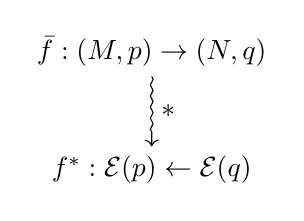
\begin{tikzpicture}[ node distance=1.5cm,
    functor/.style= {
        ->, 
        line join=round,
        decorate, 
        decoration={
            zigzag,
            segment length=4,
            amplitude=.5,
            post=lineto,
            post length=5pt
    } } ]
    \node (bar f) {$\bar f: (M,p)\to (N,q)$};
    \node (f*) [below of=bar f] {$f^*: \germs(p)\gets \germs(q)$} ;
    \draw [functor] (bar f) -- (f*)node[midway, right] {$*$};
\end{tikzpicture}
\end{center}

\subsection{Algebraist's definition}
\label{sub:algebraist_s_definition}

\begin{center}
\begin{tikzcd}[column sep=8pt]
    \bar f: (M,p) \arrow[rr, ""{name=U1, below}, "f" above] {} & & (N,q) \\
    f^*: \germs(p) \arrow[rr, phantom, ""{name=U2, below}] {} & \arrow[rightsquigarrow, from=U1, "*", end anchor={[yshift=3pt]}]& \arrow[ll] \germs(q) \\
    T_p f: T_p M \arrow[rr, ""{name=U3, below}] {} & \arrow[rightsquigarrow, from=U2, "T",end anchor={[yshift=3pt]}] & T_q N 
\end{tikzcd}

\end{center}

\subsection{Physicist's definition}
\label{sub:physicist_s_definition}
\subsection{Geometer's definition}
\label{sub:geometer_s_definition}



\chapter{Lie Groups}
\label{cha:lie_groups}

\section{Overview}
\label{sec:overview}

\begin{enumerate}
    \makethislistcompact
    \item Define Lie groups
    \item Two principles
    \item Vector fields, differential forms
    \item The Lie bracket: two ways to define it.
    \item The transition: Lie groups $\to$  Lie algebras
    \item Adjoint representation
    \item Examples of Lie algebras - from classical groups
    \item Exponential map
    \item Apply the exponential map to Lie groups
\end{enumerate}




\chapter{Campbell-Baker-Hausdorff}
\section{}
We describe the algebraic proof of the CBH formula. 

\begin{enumerate}
    \makethislistcompact
    \item Define universal enveloping algebra
    \item Define the tensor algebra
    \item Show that universal enveloping algebra and the tensor algebra are canonically isomorphic
    \item Poincaré-Birkhoff-Witt theorem
\end{enumerate}

\subsection{Universal enveloping algebra}
\label{sub:universal_enveloping_algebra}

A \emph{universal enveloping algebra} is, in some sense, the most general associative algebra which contains a given lie algebra. 

Let $U(L)$ be an associative algebra with unit and $L$ be a lie algebra. $U(L)$ is the universal enveloping algebra if we have a map $\epsilon: L\to U(L)$ such that
\begin{enumerate}
    \makethislistcompact
    \item $\epsilon$ is Lie algebra homomorphism. This means that it is linear and it preserves the Lie bracket:
        \begin{align}
            \epsilon[x,y] &= \epsilon(x)\epsilon(y) - \epsilon(y) \epsilon(x)
        \end{align}
    \item it satisfies a \emph{universal property}. If $A$ is any associative algebra with unit and $\alpha: L \to A $ is any Lie algebra then there exists a unique $\phi: U(L)\to A$ such that the following diagram commutes.
        \begin{center}
            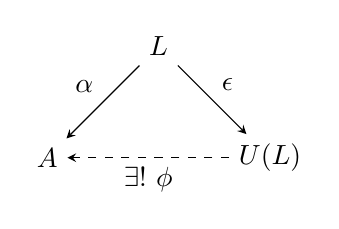
\begin{tikzpicture}[commutative diagram]
                \node (L) {$L$};
                \node (UL) [below right of=L] {$U(L)$};
                \node (A) [below left of=L] {$A$};
                \draw [arrow] (L) --(UL) node [midway, auto=left] {$\epsilon$};
                \draw [arrow] (L) --(A) node [midway, auto=right] {$\alpha$};
                \draw [arrow, dashed] (UL) --(A) node [midway, auto=below] {$\exists!\ \phi$};
            \end{tikzpicture}
        \end{center}
\end{enumerate}
\begin{insight}
    Given $(\epsilon_1, U_1)$ and $(\epsilon_2,U_2)$ we can see get maps $\phi_1: U_1\to U_2$  and $\phi_2: U_2\to U_1$ such that 
    $\phi_1\cdot\phi_2$ is identity \Todo{on $\epsilon_1(L)$} and 
    $\phi_2\cdot\phi_1$ is identity \Todo{on $\epsilon_2(L)$}. 
    But $\epsilon(L)$ generates $U(L)$, and $\phi$ is a associative algebra homomorphism, so 
    \begin{align}
        \phi\left(\sum \epsilon(x_1)\cdots\epsilon(x_n)\right) &= \sum \phi(\epsilon(x_1))\cdots\phi(\epsilon(x_n))\\
            &= \sum \epsilon(x_1)\cdots\epsilon(x_n).
    \end{align}
    Thus the compositions are identity on the whole of $U_1$ and $U_2$.
    
    %\Todo{How can we say that their composition is identity on the whole of $U_1$ and $U_2$?}
\end{insight}
Universal enveloping algebras are unique up to an isomorphism due to this universal property.

\subsection{Tensor Algebra}
\label{sub:tensor_algebra}
$i:V\to T(V)$ such that for any map $\alpha: V\to A$, where $A$ is an associative algebra, there exists a map linear map $\psi: T(V)\to A$ such that the following diagram commutes



\begin{center}
    \begin{tikzpicture}[commutative diagram]
        \node (V) {$V$};
        \node (TV) [below right of=V] {$T(V)$};
        \node (A) [below left of=V] {$A$};
        \draw [arrow] (V) --(TV) node [midway, auto=left] {$i$};
        \draw [arrow] (V) --(A) node [midway, auto=right] {$\alpha$};
        \draw [arrow, dashed] (UL) --(A) node [midway, auto=below] {$\exists!\ \psi$};
    \end{tikzpicture}
\end{center}


\subsection{Construction}
\label{sub:construction}
Let $L$ be a Lie algebra and let $I$ be the two sided ideal generated by the elements $[x,y]-x\otimes y + y\otimes x$, then
\begin{align}
    U(L) &= T(L)/I
\end{align} 
is a universal enveloping algebra for $L$.

We need to show that this satisfies the universal property. Set $V=L$ in the diagram for tensor algebra $T(V)$ to get

\begin{center}
    \begin{tikzpicture}[commutative diagram]
        \node (L) {$L$};
        \node (TL) [below right of=L] {$T(L)$};
        \node (A) [below left of=L] {$A$};
        \draw [arrow] (L) --(TL) node [midway, auto=left] {$i$};
        \draw [arrow] (L) --(A) node [midway, auto=right] {$\alpha$};
        \draw [arrow, dashed] (UL) --(A) node [midway, auto=below] {$\exists!\ \psi$};
    \end{tikzpicture}
\end{center}
If, additionally, $\alpha$ is a Lie algebra homomorphism, then 
\begin{align}
    \alpha[x,y] &= \alpha(x)\alpha(y) -\alpha(y) \alpha(x)\quad\forall x,y\in L.
\end{align}
But since $\alpha=\psi\cdot i$
\begin{align}
    \psi([x,y] -x\otimes y - y\otimes x) =0
\end{align}
Therefore $I\subset \ker \psi$, and we get that there is a unique map $\overline\phi: T/I \to A$ such that the following diagram commutes

\begin{center}
    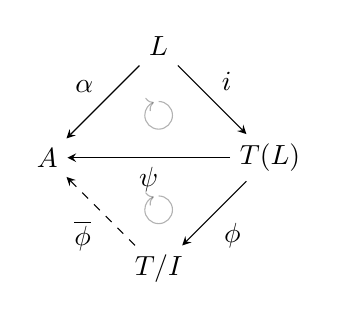
\begin{tikzpicture}[commutative diagram]
        \draw [->, opacity=0.3] (0,-0.7) arc (90:-250:5pt);
        \draw [->, opacity=0.3] (0,-1.9) arc (90:-250:5pt);

        \node (L) {$L$};
        \node (TL) [below right of=L] {$T(L)$};
        \node (A) [below left of=L] {$A$};
        \node (T/I) [below left of=TL] {$T/I$};
        \draw [arrow] (L) --(TL) node [midway, auto=left] {$i$};
        \draw [arrow] (L) --(A) node [midway, auto=right] {$\alpha$};
        \draw [arrow] (TL) --(A) node [midway, auto=below] {$\psi$};
        \draw [arrow] (TL) --(T/I) node [midway, auto=below] {$\phi$};
        \draw [arrow, dashed] (T/I) --(A) node [midway, auto=below] {$ \overline{\phi}$};
    \end{tikzpicture}
\end{center}
Thus,  we have a lie algebra $T/I$ and a map $\epsilon=\phi\cdot i: L\to T/I$ such that the universal property is satisfied. \qed



\subsection{Extension of Lie algebra homomorphism to its UEA}
\label{sub:extension_of_lie_algebra_homorphism_to_its_uea}
Given map $h: L\to M$ between two lie algebras $L$ and $M$, the universal property implies the existence of a associative algebra homomorphism $U(L)\to U(M)$ as shown in the diagram:
\begin{center}
    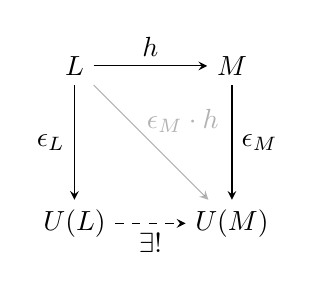
\begin{tikzpicture}[commutative diagram]
        \node (L) {$L$};
        \node (M) [right of=L] {$M$};
        \node (UL) [below of=L] {$U(L)$};
        \node (UM) [right of=UL] {$U(M)$};
        \draw [arrow] (L) -- (M) node [midway, above] {$h$};
        \draw [arrow] (L) -- (UL) node [midway, left] {$\epsilon_L$};
        \draw [arrow] (M) -- (UM) node [midway, right] {$\epsilon_M$};
        \draw [arrow, opacity=0.3] (L) -- (UM) node [midway, auto,  shift={(-5pt,0pt)}] {$\epsilon_M\cdot h$};
        \draw [arrow, dashed] (UL) -- (UM) node [midway, below] {$\exists !$};
    \end{tikzpicture}
\end{center}


\subsection{UEA of a direct sum}
\label{sub:uea_of_a_direct_sum}

\begin{align}
    U(L_1\oplus L_2) &\isomorphic U(L_1) \otimes U(L_2)
\end{align}

\subsection{Bialgebra structure}
\label{sub:bialgebra_structure}
\begin{definition}[Bialgebra]
A vector space $C$ with a map (\emph{comultiplication}) $\Delta: C\to C\otimes C$ and a map (\emph{co-unit}) $\varepsilon: D\to k$ satisfying
\begin{align}
    (\varepsilon\otimes \id) \circ \Delta &= \id \quad\text{and} \\
    (\id\otimes \varepsilon) \circ \Delta &= \id
\end{align}
is called a \emph{co-algebra}. If $C$ is an algebra and both $\Delta$ and $\varepsilon$ are algebra homomorphisms, we say that $C$ is a \emph{bi-algebra}.
    
\end{definition}

Let $L$ be any lie algebra. The map $f: L\to U(L)\otimes U(L)$ defined by
\begin{align}
    x\mapsto f(x)=x\otimes 1 + 1\otimes x
\end{align}
is a Lie algebra homomorphism. This can be seen by
\begin{align}
    f(x)f(y)- f(y)f(x) &= [x,y]\otimes 1 + 1\otimes [x,y]\\
        &= f[x,y].
    %f([x,y]) &= f(x\otimes y - y\otimes x) 
\end{align}
Thus this map induces a map $\Delta: U(L)\to U(L)\otimes U(L)$ as seen in the following commutative diagram.
\begin{center}
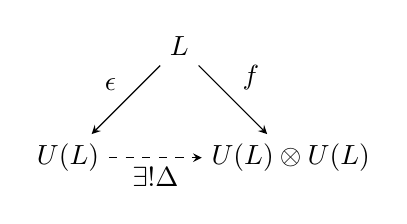
\begin{tikzpicture}[commutative diagram]
    \node (L) {$L$};
    \node (ULxUL) [below right of=L] {$U(L)\otimes U(L)$};
    \node (UL) [below left of=L] {$U(L)$};
    \draw [arrow] (L) -- (ULxUL) node [midway, auto=left] {$f$};
    \draw [arrow] (L) -- (UL) node [midway, auto=right] {$\epsilon$};
    \draw [arrow, dashed] (UL) -- (ULxUL) node [midway, below] {$\exists! \Delta$};
\end{tikzpicture}
\end{center}
Now, define the map $\varepsilon: U(L)\to k$ as
\begin{equation}
    \epsilon(x) = \begin{cases} 
        1 &\text{if } x=1,\\
        0 &\text{for all } x\in L
    \end{cases}
\end{equation}
and extend this as an algebra homomorphism.
\begin{proposition}
   $(U(L), \Delta, \varepsilon)$  is a bialgebra.
\end{proposition}
\begin{proof}
    \Todo{complete this} 
\end{proof}

\subsection{The Poincar\'e-Birkhoff-Witt Theorem.}
\label{sub:the_poincar'e_birkhoff_witt_theorem_}

\Todo{Complete this section.}

\begin{theorem}[Poincar\'e-Birkhoff-Witt]
    \begin{align}
        S(L) \isomorphic \gr U(L)
    \end{align}
\end{theorem}




\chapter{Lie Algebras}
\label{cha:lie_algebras}
In this chapter, we undertake a systematic study of Lie algebras and attempt to classify them.

\section{Definitions}
%\label{sec:definitions}

Let's make a few definitions.
\begin{align}
    D\LieG &= [\LieG, \LieG] &\text{}\\
    D_k\LieG &= [\LieG, D_{k-1}\LieG] &\text{lower central series}\\
    D^k\LieG &= [D^{k-1}\LieG, D^{k-1}\LieG] &\text{derived series}
\end{align}

\begin{definition} A lie algebra $\LieG$ is 
    \begin{enumerate}[(i)]
        \makethislistcompact
        \item \textbf{nilpotent} if $D_k\LieG=0$ for some $k$,
        \item \textbf{solvable} if $D^k\LieG=0$ for some $k$, and
        \item \textbf{semi-simple} if it has no non nonzero solvable ideals.
    \end{enumerate}
\end{definition}

\begin{definition}[Radical]
    Sum of all solvable ideals in $\LieG$ is again a solvable ideal, called the \textbf{radical} of $\LieG$ and denoted by $\Rad(\LieG)$. This is the maximal solvable ideal.
\end{definition}

\begin{lemma}[Equivalent definitions of a semisimple Lie algebra]
    \label{lemma:semisimple_definitions}
    A Lie algebra is semisimple iff 
    \begin{enumerate}[(i)]
        \makethislistcompact
        \item it has no non zero solvable ideals;
        \item $\Rad \LieG=0$;
        \item it has no non-zero abelian ideals.
    \end{enumerate}
\end{lemma}
\begin{proof}
    The first two are obvious. We will prove that they are equivalent to the third.
    Let $\LieG$ be a semisimple Lie algebra. It does not contain any non zero abelian ideal since abelian ideals are solvable. On the other hand, if it is not semisimple, then let $\Lie r = \Rad \Lie g \neq 0$. Since $\Lie r$ is solvable, $D^k\Lie r = [D^{k-1}\Lie r, D^{k-1}\Lie r]=0$ for some minimum $k$. $D^{k-1}\Lie r$ is thus an abelian ideal.

\end{proof}

\begin{definition}[Reductive]
    A lie algebra $\LieG$ is \textbf{reductive} if it is the direct sum of a semisimple lie algebra and an abelian lie algebra.
\end{definition}
\begin{insight}
   It does not make much sense to classify Lie algebras and keep $\Lie{gl}_n$ out of it. That's why we define reductive Lie algebras. Even though $\Lie{gl}_n$ is not semi-simple, it is reductive as $\Lie{gl}_n = \Lie{sl}_n\oplus \Lie{t}$ is the direct sum of the traceless Lie algebra with with the scalar Lie algebra.
\end{insight}

\begin{lemma}
    $ (\mathfrak{a} + \mathfrak{b})/\mathfrak{b} \isomorphic \mathfrak a / (\mathfrak a \cap \mathfrak b) $
\end{lemma}
\begin{proof} The kernel of the composite map 
   \begin{align}
       \LieA + \LieB \onto \LieA \onto \LieA/(\LieA \cap \LieB)
   \end{align} 
   is the ideal $\LieB \in \LieA + \LieB$.
\end{proof}


Notice that the lie algebra $\LieG/\Rad(\LieG)$ is semisimple. Any lie algebra fits into the exact sequence
\begin{align}
    0\to \Rad(\LieG) \to \LieG \to \LieG/\Rad(\LieG) \to 0
\end{align}
where the first algebra is solvable and the last algebra is semisimple. Our approach to classify representations of Lie  algebras is then to study the representations of solvable and semisimple Lie algebras.



\section{Overview}
%\label{sec:overview}




\begin{theorem}[Ado's theorem]
Every finite dimensional lie algebra is a subalgebra of $\LieGL(V)$.
\end{theorem}

\begin{theorem}[Lie's theorem]
    
\end{theorem}

\vspace{1em}
\hrule
\vspace{1em}

Reference: FH 8.3
\begin{proposition}
    Let $G$ be a Lie group and $\LieG$ be the its Lie algebra. Let $\LieH\in \LieG$ be a subalgebra. 
    Then the subgroup of $G$ generated by $\exp(\LieH)$ is an immersed subgroup $H$ with tangent space $T_eH=\LieH$
\end{proposition}
\begin{proof}
    \Todo{complete this.} 
\end{proof}


\begin{insight}
    Let $\{(e^{\iota \alpha t}, e^{\iota\beta t})| t\in \RR\} \subseteq S^2 $. This is dense in $S^2$ if $\alpha/\beta$ is irrational. So, it's not closed. It's important to keep in mind the difference in closed and immersed groups. 
\end{insight}



\section{Covering Space}
\label{sec:covering_space}

\begin{figure}[h]
    \centering
    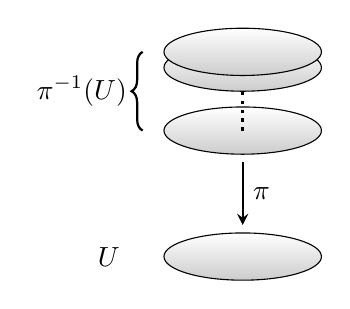
\begin{tikzpicture}[disc/.style={top color=white, bottom color=white!80!black}]
        \def\dist{0.2}
        \def\xrad{1}
        \def\yrad{0.3}
        \draw [disc] (0,-13*\dist) ellipse [start angle=0, end angle=360, x radius=\xrad, y radius=\yrad] node (U) {};
        \draw [-stealth, thick] (0,-7*\dist) -- (0,-11*\dist) node [midway, right] {$\pi$};
        \draw [disc] (0,-5*\dist) ellipse [start angle=0, end angle=360, x radius=\xrad, y radius=\yrad] node (bottom) {};
        \draw [dotted, very thick] (0,-5*\dist) -- (0,-\dist);
        \draw [disc] (0,-\dist) ellipse [start angle=0, end angle=360, x radius=\xrad, y radius=\yrad];
        \draw [disc] ellipse [start angle=0, end angle=360, x radius=\xrad, y radius=\yrad] node (top) {};

        \node [left of=U, node distance=1.7cm] {$U$};

        %\begin{scope}[shift={(-1.5cm,0cm)}]
        %\draw [decorate, decoration={brace, mirror, amplitude=2pt}] node [left of=top, node distance=1.5cm] {} -- node [left of=bottom] {};
        \def\xx{1.2cm}
        \draw [decorate, decoration={brace, mirror, amplitude=4pt, raise=2pt}, thick] ($(top)- (\xx,0)$) -- ($(bottom) - (\xx,0)$) node [midway, left, xshift=-4pt] {$\pi^{-1}(U)$};
        %\end{scope}

    \end{tikzpicture}
\end{figure}

A covering space is a space $C$ with a continuous \emph{surjective} map 
\begin{align}
    \pi: C\to X
\end{align}
such that for any point $x\in X$, there exists an open neighbourhood $U$ of $x$ such that 
\begin{align}
    \pi^{-1}(U)   &=  \coprod U_\alpha \quad\text{and}\\
    \pi|_{U_\alpha}&: U_\alpha \xrightarrow{\isomorphic} U
\end{align}
where the $U_\alpha$ are open sets and $\coprod$ is the disjoint union.
\begin{insight}
    Example 
    \begin{align}
        \RR\onto \RR/\ZZ
    \end{align}
    Every quotient is not a cover.
\end{insight}

\subsection{Universal Cover}
\label{sub:universal_cover}


A covering space is a \emph{universal covering space} if it is simply connected. 

It is universal in the sense that if there is any other cover $C$ of $X$, then there is a covering map $f: D\to C$ such that following diagram commutes
\begin{center}
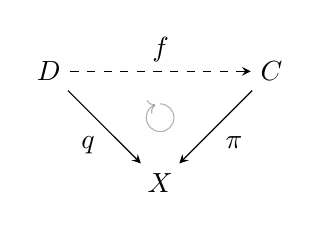
\begin{tikzpicture}[commutative diagram]
    \node [] (X) {$X$};
    \node [above left of=X] (D) {$D$};
    \node [above right of=X](C) {$C$};

    \draw [arrow] (D) -- (X) node [midway, auto=right] {$q$};
    \draw [arrow, dashed] (D) -- (C) node [midway, above] {$f$};
    \draw [arrow] (C) -- (X) node [midway, auto=left] {$\pi$};

    \draw [->, opacity=0.3] (0,1) arc (90:-250:5pt);

    
\end{tikzpicture}
\end{center}

\begin{insight}
   The universal cover of the space $X$ covers all the connected covers of the space $X$.
\end{insight}

\subsection{Second Principle}
\label{sub:second_principle}

Let $G$ and $H$ be Lie groups, $G$ is simply connected. Let $\LieG, \LieH$ be the associated Lie algebras. A linear map $\alpha: \LieG \to \LieH$ is the differential of a map $A: G\to H$ of Lie groups if and only if $\alpha$ is a map of Lie algebras.

\begin{proposition}
   A linear map $\alpha: \LieH \to \LieG$  is an isomorphism iff $A: H\to G$ is an isogeny.
\end{proposition}

\begin{proof}  {[\Todo {Sanitize; Lecture 10.17.2014}]} \\
Isogeny implies that there exists a $U\ni I_h$, such that
\begin{align}
    \varphi|_U : U_h \xrightarrow{\ \isomorphic\ } \varphi(U_h)
\end{align}
is an isomorphism.
Suppose, conversely, that $d\varphi: \LieH\to \LieG$ is an isomorphism. Then there exists a neighbourhood $U\ni I_h$ such that $    \varphi: U\to \varphi(U)$ is an isomorphism.

\begin{align}
    \varphi^{-1} (I_g) &= \bigcup_\alpha h_\alpha 
\end{align}
If $h_\alpha \neq I$, then $h_\alpha \not\in U$. Therefore, $\bigcup h_\alpha$ is a disjoint union.


Then $\coprod_\alpha U h_\alpha h\to \varphi(U)g$  is the cover of $U_g$ whenever $\varphi(h)=g$.

\end{proof}

\subsection{A bit on isogeny}
\label{sub:a_bit_on_isogeny}

Let $G$ be a group, $H$ a connected manifold. Let $\varphi: H\to G$ be a covering space map. Let $e' \mapsto e_G$. Then there exists a unique Lie group structure on $H$ such that  $e' = \id_H$ and $\varphi: H\to G$ is a Lie group morphism.

\begin{proposition}
   Let   
\end{proposition}

\begin{proof}[Proof of Second Pricniple]
    \Todo{Complete this}
\end{proof}

\section{Rough Classification of Lie Algebras}
\label{sec:rough_classification_of_lie_algebras}

We have three major theorems in this section:
\begin{enumerate}
    \makethislistcompact
    \item Engel's theorem,
    \item Lie's theorem,
    \item Levi decomposition theorem,
    \item Ado's theorem
\end{enumerate}

\subsection{Levi decomposition}
\label{sub:levi_decomposition}

We have the short exact sequence
\begin{align}
    \Rad \LieG \hookrightarrow \LieG \onto \LieG/\Rad\LieG
\end{align}
Levi's theorem basically states that this sequence splits, that is, there is an subspace $\Lie{l}$ such that
\begin{align}
    \LieG = \Lie{l}\oplus\Rad\LieG
\end{align}

\hrule\vspace{1em}
\Todo{Sanitize; Lecture 10.17.2014}

\begin{theorem}[Levi's theorem]
   Let $\LieG$  be a lie algebra with the radical $\Lie r$. There exists a subalgebra $\Lie l$ such that $\Lie g = \Lie l \oplus \Lie r$.
\end{theorem}
\begin{insight}
    This looks very much like 
    \begin{align}
        \begin{pmatrix}  x& y \\ 0 & z \end{pmatrix} &= \begin{pmatrix} x & 0 \\ 0 & z \end{pmatrix} + \begin{pmatrix} 0 & y \\ 0 & 0  \end{pmatrix}
    \end{align} 
\end{insight}
\begin{proof}
    Reduction step: No non-zero ideal is properly contained in $\Lie r$. (Otherwise if $\Lie i\subset \Lie r$ then $\Lie r/\Lie i \in \Lie g/ \Lie l$) 
     In particular, we can assume that $\Lie r $ is abelian (otherwise $0\neq D\Lie r\subset \Lie r$).

     $D\Lie r$ is preserved by all derivations of $\LieG$ (that is, all linear maps $LieG\to LieG$ satisfying the Leibniz rule). In particular, $D\Lie r$ is a radical of $\LieG$.
     So, $\Lie r$ is abelian. We may also assume that $[\Lie g, \Lie r]\neq 0$ (otherwise, )
    
    \Todo{....Complete this}.

    
\end{proof}

\subsection{Engel's theorem}
\label{sub:engel_s_theorem}

\begin{theorem}[Engel's theorem]
    Let $\LieG\in \LieGL(V)$ be any Lie subalgebra such that every $X\in \LieG$ is a nilpotent endomorphism of $V$. Then there exists a nonzero vector $v\in V$ such that $X(v)=0$ for all $X\in\LieG$.
\end{theorem}
\begin{corollary}
    
\end{corollary}
    This implies that there exist a basis in which $\LieG$ is upper triangular.

\subsection{Lie's Theorem}
\label{sub:lie_s_theorem}
\begin{theorem}[Lie's Theorem]
    Let  $\LieG\in\LieGL(V)$ be a complex solvable Lie algebra. Then there exists a nonzero vector $v\in V$ that is an eigenvector of $X$ for all $X\in \LieG$.
\end{theorem}

\section{Complete Reducibility aka Semisimplicity}
\label{sec:complete_reducibility_aka_semisimplicity}

\Todo{Lecture 10.22.2014}

\begin{definition}[Semisimplicity]
    A representation of a group or a Lie algebra is \emph{semisimple} if given a subrepresentation $W\in V$, there exists another invariant subspace $W'\in V$ such that $W\cup W'=\varnothing$ and $V=W\oplus W'$. 

In such a case, $W'$ is said to be complement to $W$.
\end{definition} 


\begin{insight}
    As an example of a Lie algebra which is not semisimple, consider the Borel algebra defined as
    \begin{align}
        B= \left\{ \begin{pmatrix} x & y \\ 0 & z \end{pmatrix} \in \GL_2(\RR)\right\} .
    \end{align}
    The vector $ \begin{pmatrix} 1 \\ 0 \end{pmatrix}$ spans an invariant subspace but has no complement.
\end{insight}

\subsection{Killing Form}
\label{sub:killing_form}

\begin{itemize}
    \makethislistcompact
    \item \Todo{Lecture 10.22.2014}
    \item \cite{humphreys1972introduction} Section II.4
    \item \cite{fulton_representation_1991} Section 14.2
\end{itemize}

\Todo{Lecture on 10.24.2014}

\begin{proposition}
    A Lie algebra is semisimple iff the Killing form is degenerate.
\end{proposition}
\begin{proof}
    \Todo{Complete this}
\end{proof}

We have two notions of semisimplicity. One is the direct sum of simpler objects, and the other one is \Todo{...}. The following corollary talks about about the first notion.
\begin{corollary}
   A semisimple Lie algebra is a direct product of simple Lie algebras. (This implies that $\LieG=D\LieG$ if $\LieG$ is a semisimple Lie algebra.)
\end{corollary}
\begin{proof}
    For any ideal $\LieH \subset \LieG$, 
    \begin{align}
        \LieH^\dagger = \{x\in \LieG\ |\  B(x,\LieH)=0 \}
    \end{align}
    is an ideal, since $ B([x,y],\LieH) = B(x,[y,\LieH]) \subset B(x,\LieH) = 0$. By Cartan's criterion, $\LieH^\dagger\cap \LieH$ is solvable, but $\LieG$ is semisimple, so $\LieH^\dagger\cap\LieH=0$. \Todo{Complete this.}
\end{proof}


\subsection{Complete Reducibility}
\label{sub:complete_reducibility}
A $\LieG$-module $V$ is called \emph{completely reducible} if $V$ is a direct sum of irreducible $\LieG$-submodules, or equivalently, if each $\LieG$-submodule $W\subset V$ has a complement $W'\in W$.




\begin{theorem}[Weyl's Theorem]
    \label{thm:weyl}
    Finite dimensional reprsentations of a semisimple Lie algebra are completely reducible. 

    Equivalently, let $V$ be a representation of a semisimple Lie algebra $\LieG$. Let $W\subset V$ be a submodule. There exists a complement $W'$, that is, a subrepresentation $W'\subset V$ such that $W+W'=V$ and $W\cap W'=0$.
\end{theorem}
\begin{proof}
   Introduce the Casimir operator. \Todo{Complete this.}
\end{proof}

\begin{insight}
   %Another approach to complete reducibility 
   Representations of $\SL_n(\CC)$ are the same as representations of $\SU_n(\RR)$. Notice that even though $\SU_n(\RR) \injects \SL_n(\CC)$, it is \emph{not} a complex Lie group. It is a real Lie group.
   \Todo{More to come...}
\end{insight}

\subsection{Jordon-Chevalley Decomposition}
\label{sub:jordon_chevalley_decomposition}

\emph{Reference: \cite{humphreys1972introduction} Section 4.2}

Here $\FF$ is a field of arbitrary characteristic.

An element $x\in \End(V)$ (for $V$ finite dimensional) is called \emph{semisimple} if the roots of its minimal polynomial over $\FF$ are all distinct. For $\FF$ an algebraically closed field, \Todo{this is equivalent to the statement that $x$ is semisimple iff $x$ is diagonalizable.}

\begin{insight}
   A Lie alegebra consisting of only semisimple elements may not be a semisimple Lie algebra.
\end{insight}

\begin{proposition}[Jordon-Chevalley Decomposition]
    Let $V$ be a finite dimensional vector space over $F$ and let $x\in \End V$. 
\begin{enumerate}[(a)]
    \item There exists a unique $x_s,\, x_n\in \End V$ satisfying the conditions: $x= x_s + x_n$, $x_s$ is semisimple, $x_n$ is nilpotent and $[x_n,x_s]=0$.
    \item There exists polynomials $p(T),\, q(T)$ in one indeterminate, without constant term, such that $x_s = p(x)$,\, $x_n = q(x)$. In particular, $x_n$ and $x_s$ commute with any endomorphism commuting with $x$.
    \item If $A\subset B \subset V$ are subspaces, and $x$ maps $B$ into $A$, then $x_s$ and $x_n$ also map $B$ into A.
\end{enumerate}
\end{proposition}

\subsection{Preservation of Jordon Decomposition}
\label{sub:preservation_of_jordon_decomposition}
\emph{Reference \cite{humphreys1972introduction} 6.4}

\begin{theorem}
    \label{thm:preservation_of_jordon_decomposition}
   Let $\LieG\in \LieGL(V)$  be a semisimple Lie algebra. Then $\LieG$ contains the semisimple and nilpotent parts in $\LieGL(V)$ of all of its elements. In  particular the abstract and usual Jordon decompositions coincide.
\end{theorem}

\begin{corollary}
    \label{cor:jordon}
    Let $\LieG$ be a semisimple Lie algebra. $\rho: \LieG\to \LieGL(V)$ a finite dimensional representation of $\LieG$. If $x=s + n$ is the abstract Jordon decomposition of $x\in L$, then $\rho(x)=\rho(s) + \rho(n)$ is the usual Jordon decomposition of $\rho(x)$.
\end{corollary}


\chapter{Representation theory of Lie Algebras}
\label{cha:representation_theory_of_lie_algebras}



\section{Overview}
In this chapter we'll develop the full machinery that will allow us the completely classfify the semisimple finite Lie algebras over any algebraically closed field of characteristic zero.

\begin{enumerate}[(i)]
    \makethislistcompact
    \item Irreps of $\SL_2$
    \item General semisimple case
    \item Root space decomposition
    \item Cartan subalgebra
\end{enumerate}


\section{Irreps of \texorpdfstring{$\mathfrak{sl}_2$}{sl\_2}}
\label{sec:irreps_of_sl_2}

Let $\LieG=\LieSL(2,\FF)$ and $V$ be an arbitrary $\LieG$-module.
%Let $V$ be a $\SL_2$ module.

Choose
\begin{align}
    X = \begin{pmatrix} 1 & 0 \\ 0 & 0 \end{pmatrix}, \quad
    Y = \begin{pmatrix} 0 & 0 \\ 0 & 1 \end{pmatrix}, \quad
    H = \begin{pmatrix} 1 & 0 \\ 0 & -1 \end{pmatrix}.
\end{align}
Computing the commutators, we get
\begin{align}
    [H,X] = 2X,\quad [H,Y]=-2Y,\quad [X,Y]=H.
\end{align}
\Todo{$H$ acts diagonally on $V$, by corollary~\ref{cor:jordon}. Since $H$ is diagonalizable iff the eigenspaces span the vector space...}

We have the eigenspaces
\begin{align}
    V_\lambda = \{v\in V\ |\ H v = \lambda(v) v\}
\end{align}
where $\lambda(v)\in \FF$. This yields the decomposition
\begin{align}
    V &= \bigoplus_{\lambda\in \LieH^*} 
\end{align}
This yields a decomposition of $V$ as direct sum of eigenspaces 

When $V_\lambda \neq \{0\}$, we call $\lambda$ a weight of $H$ in $V$ and we call $V_\lambda$ a weight space.

\begin{lemma}
    If $v\in V_\lambda$ then $Xv \in V_{\lambda + 2}$ and $Yv\in V_{\lambda-2}$.
\end{lemma}
\begin{proof} Trivial.
\end{proof}
Finite dimensionality of $V$ implies the existence of a maximal $\lambda$. For such $\lambda$, any nonzero vector in $V_\lambda$ is called a \emph{maximal vector of weight $\lambda$}.

\subsection{Classification of irreducible modules}
\label{sub:classification_of_irreducible_modules}

Assume now that $V$ is an irreducible $\LieSL_2$ module. Choose a maximal vector $v_0\in V_\lambda$ and set
\begin{align}
    v_{-1}&=0, \\
    v_k &= \frac{1}{k!} Y^k v_0, \quad\text{for } k\geq 0.
\end{align}

\Todo{more stuff here...}

\section{Root Space Decomposition}
\label{sec:root_space_decomposition}

Let $\LieG$ be a semisimple Lie algebra.

\begin{definition}
    A Lie subalgebra $\Lie t \subset \Lie g$ is \emph{toral} if it contains only semisimple elements.
\end{definition}

\begin{insight}
    Where is the torus in the toral Lie algebra? 
\end{insight}

\begin{lemma} 
    Toral subalgebras exist.
\end{lemma}
\begin{proof}
    Every element $x\in \LieG$ can be decomposed as into nilpotent and semisimple parts $x=x_s + x_n$, which are also in $\LieG$. 
    If there was no semisimple element in $\LieG$, that is, if all the elements were nilpotent then $\LieG$ would be a nilpotent Lie algebra (by Engel's theorem). A semisimple Lie algebra can not be nilpotent (since nilpotent implies solvable). So, there exists some subalgebra (span of the semisimple elements) which is toral.
\end{proof}

\begin{lemma}
    A toral subalgebra is abelian.
    \label{lemma:toralsubalgebra_abelian}
\end{lemma}
\begin{proof}
    Let $\Lie t \subset \Lie g$ be a toral subalgebra. We need to show that $\ad_{\Lie t} x=0 $ for all $x\in \Lie t$. Since $x\in \Lie t$ is semisimple, $\ad_\Lie t x$ is semisimple and thus diagonalizable ($\FF$ is an algebraically closed field). If $\ad_\Lie t x \neq 0$, then it has linearly independent eigenvectors that span $\Lie t$. We need to show that all the eigenvalues are zero. Assume, on the contrary, that there is some non-zero $v\in \Lie t$ such that $\ad_\Lie t x (v)=av$ with $a\neq 0$. Now, notice that 
    \begin{align}
        \ad_\Lie t v(\ad_\Lie t v(x))=-a[y,y]=0
    \end{align} 
    and so $\ad_\Lie t v(x)$ is an eigenvector of $\ad_\Lie t v$ with eigenvector $0$. Since $v$ is semisimple,so is $\ad_\Lie t v$ and thus has eigenvectors that span the space. We can write $x$ as a linear combination of eigenvectors of $v$. Let $x=\sum_i a_i v_i$ where $\ad_\Lie t v (v_i)=\lambda_i v_i$ for $i=1,\dotsc,n$. Now
    \begin{align}
        \ad_\Lie t (\ad_t v(x))&= \ad_\Lie t (\sum_i a_i \lambda_i v_i) \\
            &= \sum_i a_i \lambda_i^2 v_i. 
    \end{align}
    But this must be zero, which contradicts the linear independence of the eigenvectors.  
\end{proof}

\begin{insight}
    What is the difference between Cartan subalgebras and maximal toral subalgebras?  \Todo{``Cartan subalgebra = maximal toral subalgebra'' is the correct definition only when $\Lie g$ is reductive.}
\end{insight}

\begin{definition}[Cartan subalgebra]
    The maximal toral subalgebra  is called the Cartan subalgebra.
\end{definition}

\begin{insight}
   For $\Lie {sl}(n,\FF)$, the maximal toral subalgebra is the set of all diagonal matrices.
\end{insight}
Let $\LieH$ be the Cartan subalgebra of $\LieG$. Since $\LieH$ is abelian (by lemma~\ref{lemma:toralsubalgebra_abelian}), 
\begin{align}
    [\ad_\Lie g H_1, \ad_\Lie g H_2] &= \ad_\Lie g [H_1, H_2] =0  \quad \forall H_1,\, H_2 \in \LieH.
\end{align}
So $\ad_\Lie g \Lie h$ is a commuting family of endomorphisms of $\LieG$. Therefore, $\ad_\LieG\LieH$ can be simultaneously diagonalized. In other words,
\begin{align}
    \LieG &= \bigoplus_{\alpha\in \LieH^*} \LieG_\alpha \\
    \text{with}\quad \LieG_\alpha &= \{x\in \LieG\ |\ \ad_\LieG h (x)=\alpha(h)x \quad\forall h\in \LieH\}.
\end{align}

Notice that $\LieG_0 = \{x\in\LieG\ |\ [\LieH,x] = 0 \forall x\in\LieG\} = C_\LieG(\LieH)$, the \defn{centralizer} of $\LieH$. 
\begin{insight}
    The centralizer of a subset is the set of all elements in the group which commute with all the elements in the subset.
\end{insight}

The set of all nonzero $\alpha\in\LieH^*$ for which $\LieG_\alpha \neq 0$ are called \defn{roots} of $\LieG$ relative to $\LieH$. We thus have the \defn{root space decomposition} or \defn{Cartan decomposition}: 
\begin{align}
    (*): \LieG &= C_\LieG(\LieH) \oplus \coprod_{\alpha\in\Phi} \LieG_\alpha
\end{align}

\chapter{Root Systems}
\label{cha:root_systems}

A \defn{Euclidean space} is is a vector space $E\isomorphic \RR^n$ equipped with a positive definite symmetric bilinear form $(\cdot,\cdot): E\times E \to \RR$. A reflection about any nonzero vector $\alpha$ is defined as
\begin{align}
    \sigma_\alpha(\beta) &= \beta - 2 \frac{(\beta,\alpha)}{(\alpha,\alpha)} \alpha
\end{align}
with the reflecting hyperplane given by
\begin{align}
    P_\alpha &= \{\beta\in E \ |\ (\beta,\alpha)=0\}.
\end{align}
We use the shorthand $\<\beta,\alpha\>=2 \frac{(\beta,\alpha)}{(\alpha,\alpha)}$.

A subset $\Phi$ of the euclidean space $E$ is called a \defn{reduced root system} in $E$ if the following axioms are satisfied:
\begin{enumerate}[(R1)]
    \makethislistcompact
    \item $\Phi$ is finite, spans $E$ and $\Phi\not\ni 0$.
    \item If $\alpha\in \Phi$, the only multiples of $\alpha$ in $\Phi$ are $\pm \alpha$.
    \item If $\alpha\in\Phi$, the reflection $\sigma_\alpha$ leaves $\Phi$ invariant.
    \item If $\alpha,\beta\in \Phi$, then $\<\beta,\alpha\>\in \ZZ$
\end{enumerate}

\begin{insight}
    If axiom (R2) is removed, then we get a \defn{root system} (no longer \emph{reduced}). This is useful in the classification of real semisimple Lie algebras.
\end{insight}

Let $\Phi$ be a root system in $E$. Let $\Weyl$ denote the subgroup of $\GL(E)$ generated by the reflections $\sigma_\alpha$. 

By (R3), $\Weyl$ permutes the set $\Phi$, which by (R1).
$\Weyl$ is the Weyl group.

\begin{lemma}
    Let $\Phi$  be a root system in $E$, with Weyl group $\Weyl$. If $\sigma\in \GL(E)$ leaves $\Phi$ invariant, then $\sigma \sigma_\alpha \sigma^{-1} = \sigma_{\sigma(\alpha)}$ for $\alpha\in \Phi$ and $\<\beta,\alpha\>=\<\sigma(\alpha),\sigma(\beta)\>$  for all $\alpha,\beta \in \Phi$.
\end{lemma}
\begin{proof}
    
\end{proof}

\section{Bases}
\label{sec:bases}

A subset $\Delta \subset \Phi$ is called a \defn{base} if:
\begin{itemize}
    \makethislistcompact
    \item [(B1)] $\Delta$ is a basis of $E$
    \item [(B2)] each root $\beta$ can be written as a $\beta = \sum k_\alpha \alpha$ with $\alpha\in \Delta$ with integral coefficients all non-negative or nonpositive.
\end{itemize}

\begin{insight}
   \begin{lemma}
       A root is simple if and only if it cannot be written as a sum of other roots.
   \end{lemma} 
   \begin{proof}
       \Todo{Prove this.} 
   \end{proof}
\end{insight}

The roots in $\Delta$ are called \defn{simple} (\Todo{Is the definition of simple relative to the base?}).
\Todo{Is Card $\Delta$= Dim $\Delta$}? 
Since $\Delta$ is a basis, the expression given by (B2) is unique. This lets us define the \defn{height} of a root (relative to $\Delta$) by 
\begin{align}
    \height \beta = \sum_{\alpha\in \Delta} k_\alpha
\end{align}
A root is \defn{positive} if all $k_\alpha\geq0$ and \defn{negative} if all $k_\alpha<0$. The set of all positive roots is denoted by $\Phi^+$ and the set of all negative roots is given by $\Phi^-$.

We need to show that a base defined as above actually exists. We do this by explicit construction. But first, we need 
\begin{lemma}
    If $\Delta$ is a base of $\Phi$, then $(\alpha,\beta)\leq 0$  for all $\alpha\neq\beta$ in $\Delta$, and $\alpha-\beta$ is not a root.
\end{lemma}
\begin{proof}
    We have, by an earlier lemma (\Todo{reference}) that if $(\alpha,\beta)>0$ then $\alpha - \beta$ is a root. The logical negation of that statement is that if $\alpha + \beta$ is not a root, then $(\alpha,\beta)\leq 0$. But $\alpha-\beta$ can not be a root since that would violate that the second axiom (B2) that all coefficients must have the same sign.
\end{proof}
\begin{theorem}
    Bases exist.
\end{theorem}
    For a vector $\gamma\in E$, define 
    \begin{align}
        \Phi^+(\gamma) = \{\alpha\in\Phi\ |\ (\gamma,\alpha)>0\}.
    \end{align}
    This is just the set of all vectors lying to the \emph{positive} side of the hyperplane orthogonal to $\gamma$, given by $P_\gamma$. 
    \begin{insight}
        Any finite union of hyperplanes in a euclidean space cannot exhaust all of the space. If you hyperplanes corresponding to vectors $S=\{\alpha_1,\dotsc,\alpha_n\}$, take a linearly independent subset of $S$ that spans $\<S\>$. The number of vectors in the subset must be less than or equal to $\dim E$. \Todo{Complete this}
    \end{insight}

    A $\gamma\in E$ is \defn{regular} if $\gamma\in E - \bigcup_{\alpha\in\Phi}P_\alpha$, \defn{singular} otherwise.

    Given a vector $\gamma$ and a root $\alpha$, you could have $(\gamma,\alpha)$ less than, greater than, or equal to 0. If it vanishes, then it is singular by definition. Now, if it is regular then all the roots are on either side of the $P_\gamma$, so $\Phi = \Phi^+(\gamma)\cup \Phi^-(\gamma)$. Call $\alpha\in \Phi^+$ \defn{decomposable} if $\alpha = \beta_1 + \beta_2$ for some $\beta_i\in \Phi^+(\gamma)$, \defn{indecomposable} otherwise.

\begin{theorem}
    Let $\gamma\in E$ be regular. Then the set $\Delta(\gamma)$  of all indecomposable roots in $\Phi^+(\gamma)$ is a base of $\Phi$, and every base is obtainable in this manner.
\end{theorem}
\begin{proof}
\end{proof}

\chapter{Conjugacy Theorems}
\label{cha:conjugacy_theorems}

References: \cite[$\S 16$]{humphreys1972introduction}

\begin{theorem}[Conjugacy of CSAs (solvable case)]
    Let $L$ be solvable. Any two CSAs are conjugate.
\end{theorem}

\defn{Borel subalgebras} are maximal solvable subalgebras of a Lie algebra $\LieG$.
\begin{lemma}
    If $B$  is a Borel subalgebra of $\LieG$, then $B=N_L(B)$.
\end{lemma}
\begin{proof}
    Let $x$ normalize $B$. Then $B + Fx$ is a subalgebra of $L$, solvable because $[B + \FF x, B + \FF x] = [B,B] + \FF [B,x] + \FF [x,B] = [B,B] \subset B$. So, $x\in B$ by maximality of $B$.
\end{proof}
\begin{insight}
    Recall that a normalizer of a group is the set of all elements that commutes with the whole group.
\end{insight}


\chapter{Cartan-Weyl Highest Weight Theory}
\label{cha:cartan_weyl_highest_weight_theory}
References: \cite[$\S 20$]{humphreys1972introduction}

In this chapter $\LieG$ denotes a semisimple Lie algebra over an algebraically closed field $\FF$ of characteristic $0$, $\LieH$ is a fixed Cartan subalgebra of $\LieG$, $\Phi$ the root system $\Delta = \{\alpha_1,\dotsc,\alpha_l\}$ a base of $\Phi$, $\Weyl$ the Weyl group.

\section{Weights and maximal vectors}
\label{sec:weights_and_maximal_vectors}

If $V$ is a finite dimensional $\LieG$-module, it follows from \Todo{Theorem~\ref{thm:preservation_of_jordon_decomposition} (preservation of Jordon decomposition)}  that $\LieH$ acts diagonally on $V$. That is 
\begin{align}
    V &= \coprod_{\lambda\in \LieH^* } V_\lambda, \quad \text{with}\\
    V_\lambda &= \{v\in V\ |\ h\cdot v = \lambda(h) v \ \forall h\in H\}
\end{align}
$V_\lambda$ is called the \defn{weight space} if $V_\lambda\neq 0$ and $\lambda$ is called a \defn{weight} of $H$ on $V$. 
These definitions make sense even when $V$ is infinite dimensional.
\begin{insight}
    Roots are just the weights of the adjoint representation, with $\LieG_\alpha$  as the weight space (dimension one).
\end{insight}

\begin{lemma}
    Let $V$ be any arbitrary $\LieG$-module. Then
    \begin{enumerate}[(a)]
        \makethislistcompact
        \item 
            $\LieG_\alpha$ maps $V_\lambda$ to $V_{\lambda+\alpha}$ for $\lambda\in \LieH^*,\,\alpha\in\Phi$
        \item 
            If $V'=\sum_{\lambda\in \LieH^*} V_\lambda$ is direct, and $V'$ is a $\LieG$-submodule of $V$.
        \item
            If $\dim V < \infty$, then $V'=V$
    \end{enumerate}
\end{lemma}
\begin{proof}
    For $x\in \LieG_\alpha$ and $v\in V_\lambda$  we have
    \begin{align*}
        h(xv) &= [h,x]v - x(hv)\\
            &= \alpha(h)xv - x\lambda(h)v \\
            &= (\alpha(h) + \lambda(h)) xv
    \end{align*}
\end{proof}

A \defn{maximal vector} (of weight $\lambda$) in a $\LieG$-module $V$ is a non-zero vector $v^+\in V_\lambda$ annihilated by all $\LieG_\alpha\ (\alpha > 0)$. 

\begin{insight}
    If $\LieG$ is simple Lie algebra and $\beta$ is a maximal root in $\Phi$ relative to $\Delta$, then any nonzero element of $\LieG_\beta$ is a maximal vector for the adjoint representation of $L$.
    If $\dim V = \infty$, then there may not be a maximal vector.
\end{insight}


A \defn{Borel subalgebra} is
\begin{align}
    B(\Delta) &= \LieH\oplus \bigoplus_{\alpha>0} \LieG_\alpha.
\end{align}
\begin{lemma}
    If $\dim V < \infty$ , then a maximal vector exists.
\end{lemma}
\begin{proof}
    \Todo{$B(\Delta)$ is a solvable subalgebra. By Lie's theorem, a solvable subalgebra contains a common eigenvector for all endomorphisms in $\LieG$.} 
\end{proof}

%By Lie's theorem, $B(\Delta)$ has a common eigenvector (killed by all \gamma_\alpha,)

A \defn{standard cyclic module} (weight $\lambda$) is a $\LieG$-module $V$ such that 
\begin{align*}
    V=U(\LieG)\cdot v^+
\end{align*}
and we call $\lambda$ the \defn{highest weight} of V. 
\begin{insight}
    The term \emph{cyclic} is often used to refer to something that is generated by one element.
\end{insight}

\begin{theorem} 
    Let $V$ be a standard cyclic $\LieG$-module, with maximal vector $v^+\in V_\lambda$. Let $\Phi^+=\{\beta_1,\dotsc,\beta_m\}$. Then
    \begin{enumerate}[(a)]
        \makethislistcompact
        \item $V$ is spanned by the vectors $y_{\beta_1}^{i_1}\cdots y_{\beta_m}^{i_m}\cdot v^+\ (i_j\in \ZZ^+)$; in particular, $V$ is the direct sum of its weight spaces.
        \item  The weights of $V$ are of the form $\mu = \lambda - \sum_{i=1}^{l}k_i \alpha_i$,  that is, all weights satisfy $\mu < \lambda$.
        \item For each $\mu \in \LieH^*$, $\dim V_\mu < \infty$ and $\dim V_\lambda = 1$.
        \item Each submodule of $V$ is the direct sum of weight spaces.
        \item V is an indecomposable $\LieG$-module, with a unique maximal (proper) submodule and a corresponding unique irreducible quotient.
        \item Every nonzero homomorphic image of $V$ is also standard cyclic of weight $\lambda$.
    \end{enumerate}
\end{theorem}

\section{Existence and uniqueness of highest weight representations}
\label{sec:existence_and_uniqueness_of_highest_weight_representations}
Reference: \cite[$\S 20.3$]{humphreys1972introduction}

\begin{theorem}
    Irreducible standard cyclic modules are isomorphic.
\end{theorem}
This theorem proves the uniqueness of highest weight representations. The next part is to prove the existence. We do this by construction.

The first type of construction is called \defn{Verma modules.}






%%%%%%%%%%%%%%%%%%%%%%%%%%%%%%%%%%%%%%%%%%%%%%%%%%%%%%%%%%%%%%%%%%%%%%%%%
% APPENDICES
%%%%%%%%%%%%%%%%%%%%%%%%%%%%%%%%%%%%%%%%%%%%%%%%%%%%%%%%%%%%%%%%%%%%%%%%%
\appendix
\chapter{Tensor Product}
\label{cha:tensor_product}

Let $V,\ W$ be vector spaces. A tensor product is a vector space $V\otimes W$ equipped with a bilinear map
\begin{align}
    V\times W \to V\otimes W\\
    (v,w) \mapsto v\otimes w
\end{align}
such that it is \emph{universal}. That is, given any other vector space $U$ and a bilinear map $\beta: V\times W\to U$, there is unique map $\beta': V\otimes W \to U$ such that $\beta'(v\otimes w) = \beta(v,w)$. The following diagram commutes:

\begin{center}
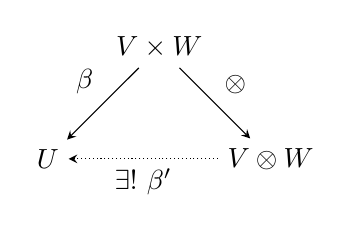
\begin{tikzpicture}[commutative diagram] 
    \node (a) {$V\times W$};
    \node (b) [below right of=a] {$V\otimes W$};
    \node (c) [below left of=a] {$U$};
    \draw [arrow] (a) -- (b) node [midway] {$\otimes$};
    \draw [arrow] (a) -- (c) node [midway,auto=right] {$\beta$};
    \draw [exists] (b) -- (c) node [midway] {$\exists!\ \beta'$};
\end{tikzpicture}
\end{center}
The universality requirement means that the tensor product thus defined is unique up to an isomorphism. Let there be another tensor product $V\otimes' W$ (a vector space and a corresponding map that takes $(v,w)\mapsto v\otimes' w$) that is also universal. Then it immediately implies that there is a bijection between $V\otimes W$ and $V\otimes' W$ since
\begin{center}
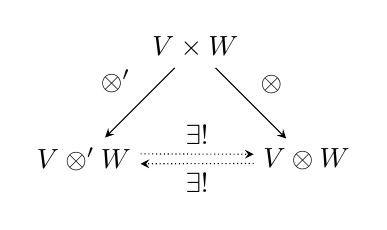
\begin{tikzpicture}[commutative diagram] 
    \node (a) {$V\times W$};
    \node (b) [below right of=a] {$V\otimes W$};
    \node (c) [below left of=a] {$V\otimes' W$};
    \draw [arrow] (a) -- (b) node [midway] {$\otimes$};
    \draw [arrow] (a) -- (c) node [midway,auto=right] {$\otimes'$};
    \draw [exists] (c.5) -- (b.175) node [midway, above] {$\exists!$};
    \draw [exists] (b.185) -- (c.355) node [midway] {$\exists!$};
\end{tikzpicture}
\end{center}

\begin{theorem}[]
    $\Hom(V,W) \isomorphic V^*\otimes W$ as vector spaces.
\end{theorem}
\begin{proof}
   Quick Check: Set $W=\CC$ so that we get $\Hom(V,\CC)\isomorphic V^*\otimes 1 = V^*$, which is the definition of the dual space $V^*$.

   Given $(\beta: V\to W) \in \Hom(V,W)$, define the map $\phi: \Hom(V,W)\to V^* \otimes W $ such that 
   \begin{align}
       \phi(\beta) = \sum_{i,j} \beta_{ij} v_i^* \otimes w_j
   \end{align}
   where $\{v_i\}$ and $\{w_j\}$ are orthonormal basis for $V$ and $W$ respectively and $\beta_{ij} = \beta(v_i)^T w_j$.
   This is a homomorphism of vector spaces. The inverse map is obvious.
\end{proof}

\section{Exterior Products and Symmetric Products}
\label{sec:exterior_products_and_symmetric_products}

\subsection{Definitions}
\label{sub:definitions}

\subsection{Some Combinatorics}
\label{sub:some_combinatorics}

Lets find out the dimensions of the vector space $\Lambda^k V$, where $V$ is an $n$-dimensional vector space.
If $\{e_i\}$ is a basis for $V$, we know that a basis for $\Lambda^k V$ is 
\begin{align}
    \{e_{i_1}\wedge e_{i_2} \wedge\cdots \wedge e_{i_k} : i_1 < i_2 < \cdots < i_k \}.
\end{align}
How many vectors are there in this basis? This can be answered by looking at how many ways are there to simply choose $k$ objects from a set of $n$ different objects. Since there is just one of arranging them (in increasing order), that would be the number of vectors in the basis. So,
\begin{align}
    \dim \Lambda^k (V) &= {}^{\dim V}C_k
    \label{eqn:dim_exteriorpower}
\end{align}

What's the dimension of $\Sym^k(V)$? The basis is
\begin{align}
    \{e_{i_1}\cdot e_{i_2} \cdot\cdots \cdot e_{i_k} : i_1 \leq i_2 \leq \cdots \leq i_k \}.
\end{align}
Another way to write that is
\begin{align}
    \{e_1^{a_1}\cdot e_2^{a_2} \cdots e_k^{a_k}\},\quad\text{such that } \sum_i a_i = n,\, a_i\geq 0.
\end{align}
We just need to know how many ways are there to distribute $n$ identical things among $k$ different people with no restriction on the number of things anyone can get. To solve this, introduce $k-1$ identical barriers (denoted by $|$) between $n$ things (denoted by $\circ$)and look at the number of permutations.
\begin{align}
    \circ | \circ | \cdots | \circ
\end{align}
Every permutation here gives possible choice of ${a_1,\dotsc,a_k}$. Therefore,
\begin{align}
    \dim (\Sym^k (V)) &= {}^{\dim V +k-1}C_{k}
    \label{eqn:dim_symmetricpower}
\end{align}


\chapter{General Information}

\section{Resources}
\label{sec:Resources}
Here are some resources that I found useful while preparing these notes
\begin{itemize}
    \item Representation Theory - A First Course by \emph{Fulton, Harris}
\end{itemize}


%%%%%%%%%%%%%%%%%%
%  Bibliography  %
%%%%%%%%%%%%%%%%%%
\nocite{*} % Print all entries in the bib file
\printbibliography

\end{document}
